\documentclass[crop,class=article]{standalone}
%----------------------------Preamble-------------------------------%
\usepackage{tikz}                       % Drawing/graphing tools.
%--------------------------Main Document----------------------------%
\begin{document}
    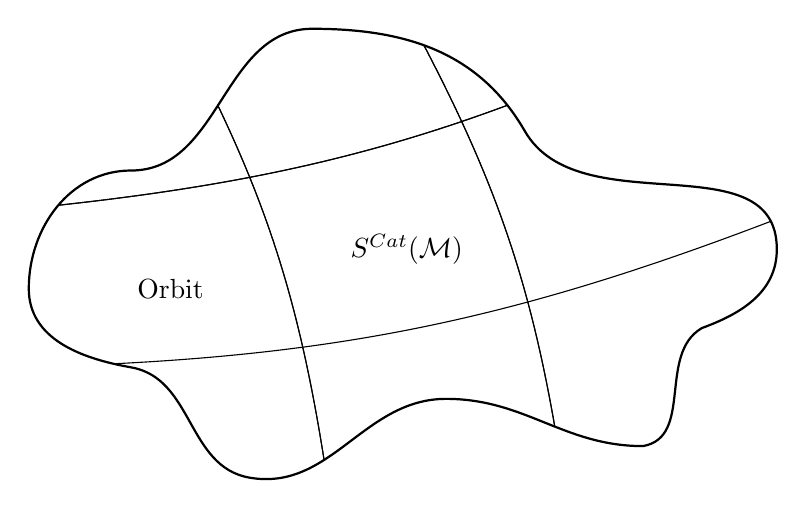
\begin{tikzpicture}
        \draw[line width=0.8pt]
            (0.2,2.5) to[out=-90,in=170]
            (1.5,1.5) to[out=-10,in=170]
            (3,0.1) to[out=-10,in=180]
            (5.5,1.1) to[out=0,in=180]
            (8,0.5) to[out=10,in=-150]
            (8.75,2) to[out=20,in=-90]
            (9.7,3) to[out=90,in=-60]
            (6.5,4.5) to[out=120,in=0]
            (3.8,5.8) to[out=180,in=0]
            (1.5,4) to[out=180,in=90] cycle;
        \clip (0.2,2.5) to[out=-90,in=170] (1.5,1.5)
                        to[out=-10,in=170] (3,0.1)
                        to[out=-10,in=180] (5.5,1.1)
                        to[out=0,in=180] (8,0.5)
                        to[out=10,in=-150] (8.75,2)
                        to[out=20,in=-90] (9.7,3)
                        to[out=90,in=-60] (6.5,4.5)
                        to[out=120,in=0] (3.8,5.8)
                        to[out=180,in=0] (1.5,4)
                        to[out=180,in=90] cycle;
        \draw (4,0) to[bend right=10] (2,6) to (5,6)
                    to [bend left=10] (7,0) to cycle;
        \draw (7,0) to[bend right=10] (5,6) to (10,6)
                    to (10,0) to cycle;
        \draw (0,1.5) to (0,3.5) to [bend right=10] (9,6)
                      to (10,6) to (10,3.5) to [bend left=10] cycle;
        \draw (0,0) to (4,0) to[bend right=10] (2,6)
                    to (0,6) to (0,0) to cycle;
        \draw (0,6) to (0,3.5) to[bend right=10] (9,6)
                    to (0,6) to cycle;
        \node at (2,2.5) {Orbit};  
        \node at (5,3) {$S^{Cat}(\mathcal{M})$};
    \end{tikzpicture}
\end{document}